\begin{subsectionframemod}{Cross-Domain Few-Shot Object Detection}

    \only<1>{
        \begin{figure}
            \centering
            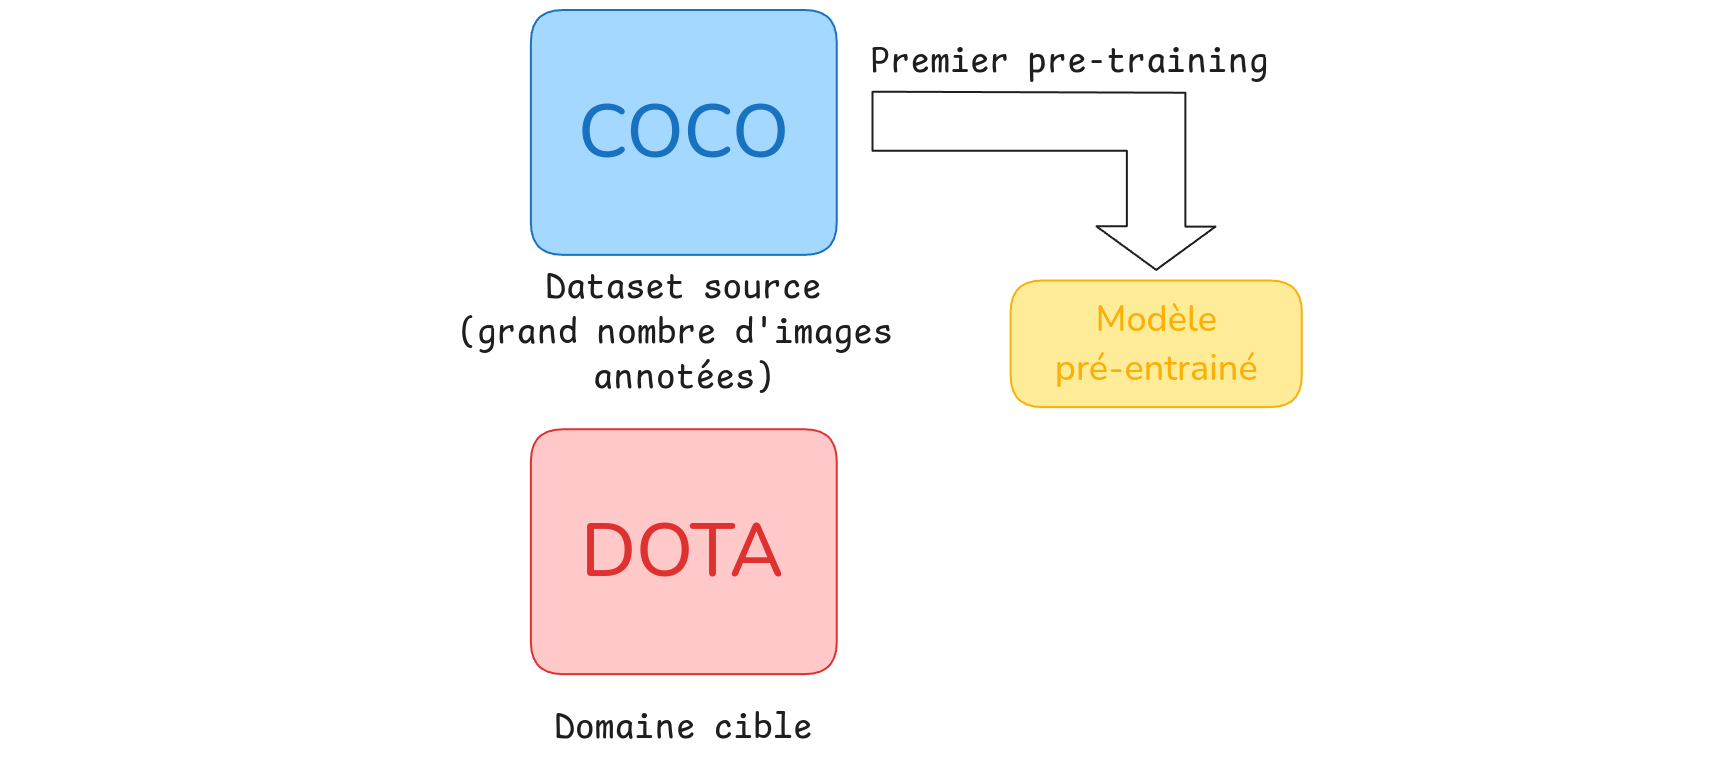
\includegraphics[width=\textwidth]{Figures/cross_domain_1}
            \caption{Schema de la méthode utilisé pour tenter d'estimer le domaine shift}
        \end{figure}
    }
    \pause
    \only<2>{
        \begin{figure}
            \centering
            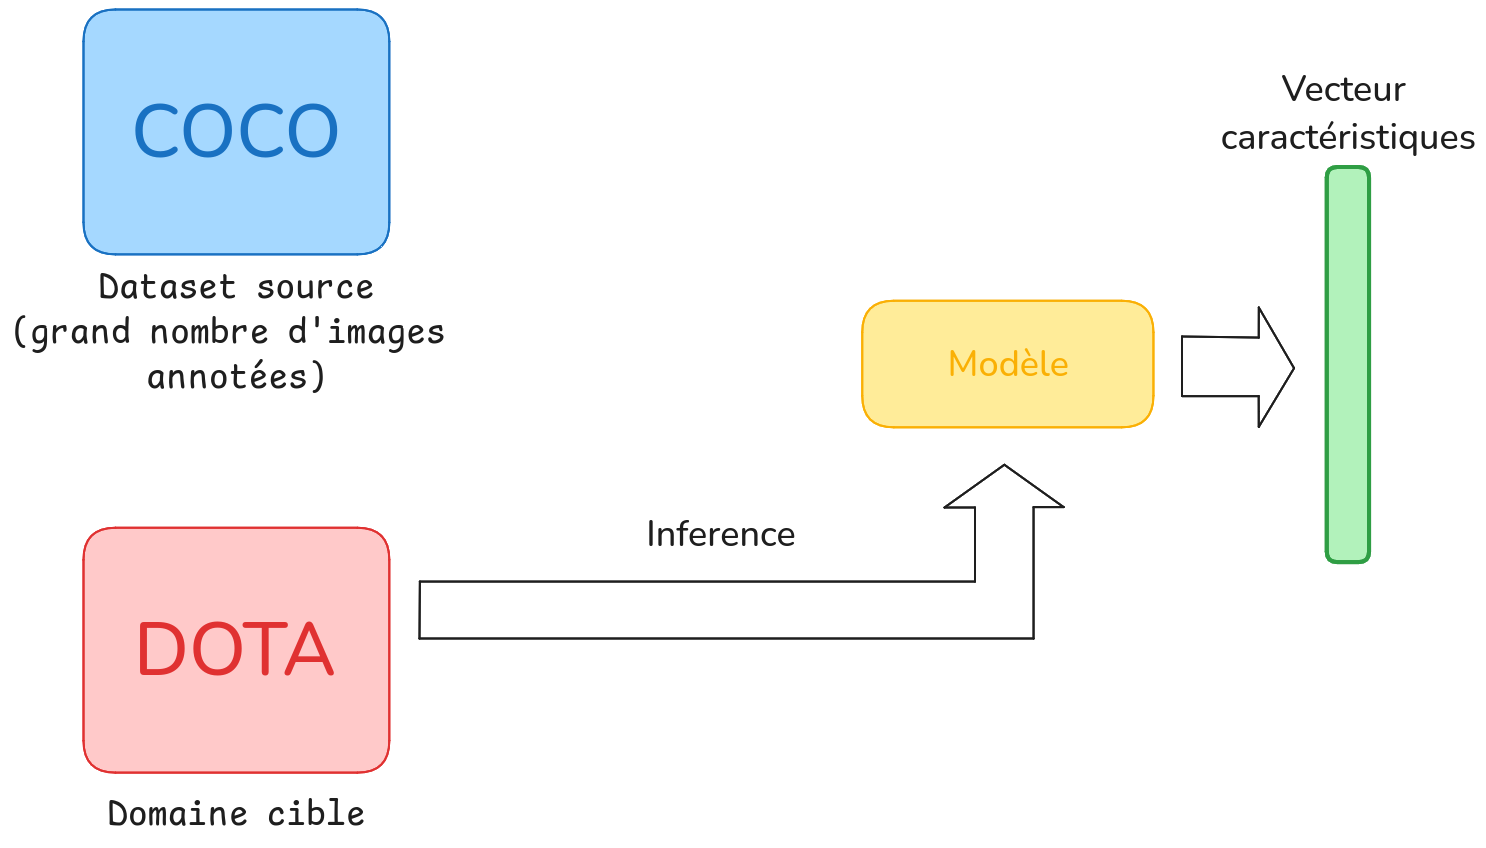
\includegraphics[width=\textwidth]{Figures/embeddings}
            \caption{Schema de la méthode utilisé pour tenter d'estimer le domaine shift}
        \end{figure}
    }
    \pause
    \only<3>{
        \begin{figure}
            \centering
            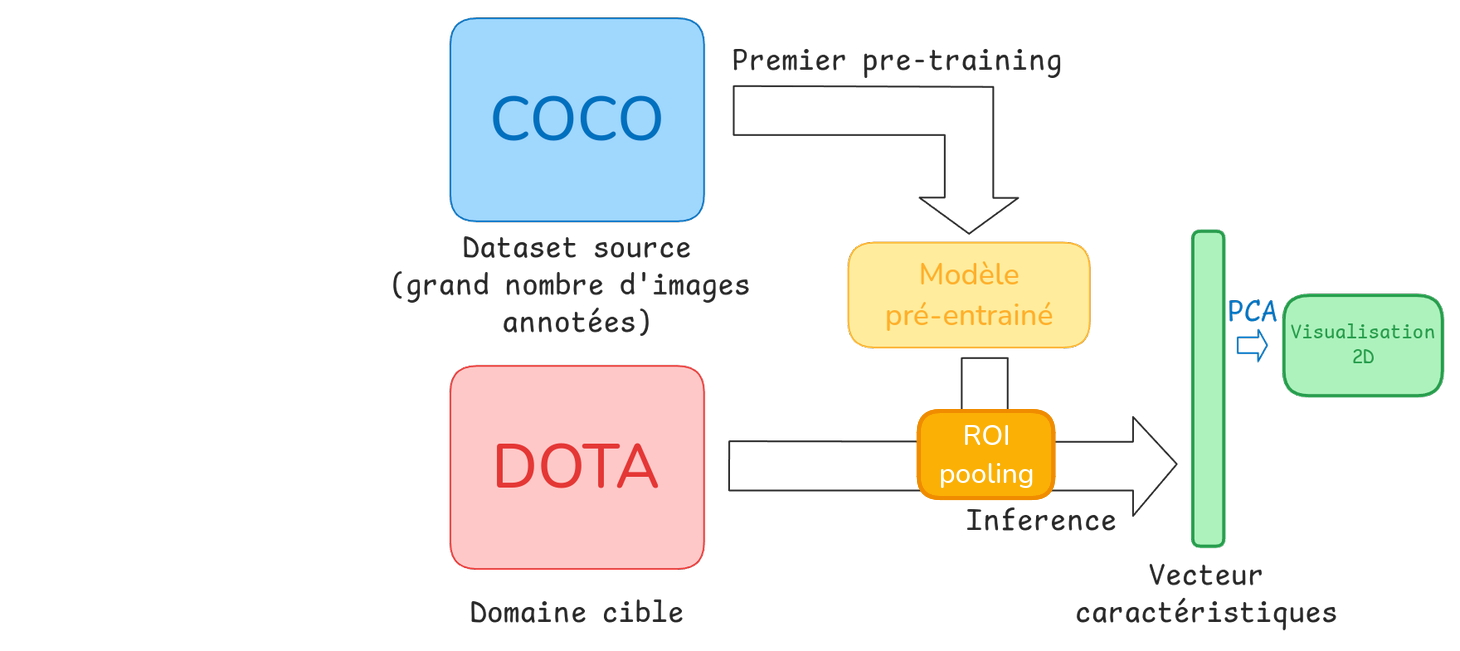
\includegraphics[width=\textwidth]{Figures/embeddings_pca}
            \caption{Schema de la méthode utilisé pour tenter d'estimer le domaine shift}
        \end{figure}
    }

\end{subsectionframemod}